% Here we have your executive summary.
This thesis describes a new method for measuring strain dependent surface stress in soft solids, as well as the corresponding measurements for two silicone polymer gels. Over the past several years, recent attempts to measure surface stress in gels have returned a cornucopia of conflicting results, differing significantly in similar materials. Recently, Xu, Jensen et al. suggested that this discrepancy is an artifact of the strain state of the gels, and made the first measurement of strain-dependent surface stress, $\Upsilon(\epsilon)$, in solids \cite{xu2017direct}. In this paper, the authors reported that the surface stress changed dramatically under applied strain. At 18\% strain, the surface stress more than doubled. 
\begin{figure}[h!]
	\centering
%	\textbf{Should I give it a title?}\par\medskip
	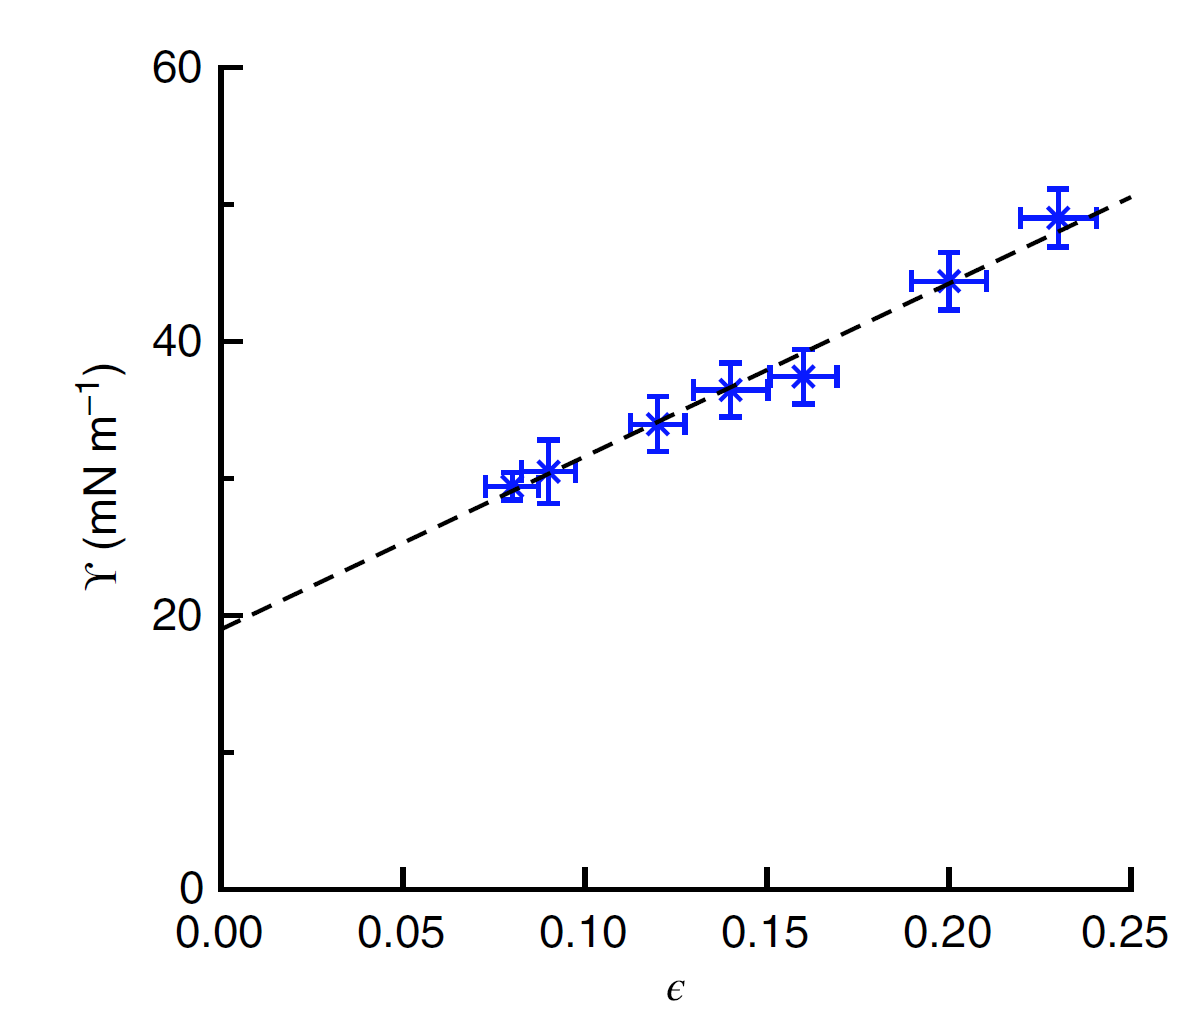
\includegraphics[width=0.7\linewidth]{Chapters/Figures/2017natcomfig}
	\caption[Surface Stress vs. Strain in Silicone]{This is first direct measurement of strain dependent surface stress in solids \cite{xu2017direct}. Using a compliant silicone gel, surface stress, $\Upsilon$, was found to grow linearly as a function of strain, $ \epsilon $.}
	\label{fig:2017natcomfig}
\end{figure}

Over the past year, we have helped develop a new method for measuring $\Upsilon(\epsilon)$ in soft solids. Our adhesion-based technique can be applied to a wide variety of stretchable materials. Additionally, we have build our own equibiaxial stretching apparatus, improving upon the earlier published design \cite{xu2017direct} to produce nearly twice the strain in identical materials. Using this technique we have measured the adhesion energy and surface stress in two types of silicone, as well as preliminary $ \Upsilon(\epsilon) $ measurements as we work towards recreate the controversial 2017 measurement.

Our results suggest that the surface tension in gels does significantly change under strain. The figure below is an example of how you can visually see this change for a single silica sphere sitting in a silicone substrate. As the underlying gel is stretched, the surface tension increases, reducing the depth into which the sphere sits. 
\begin{figure}[h!]
	\centering
	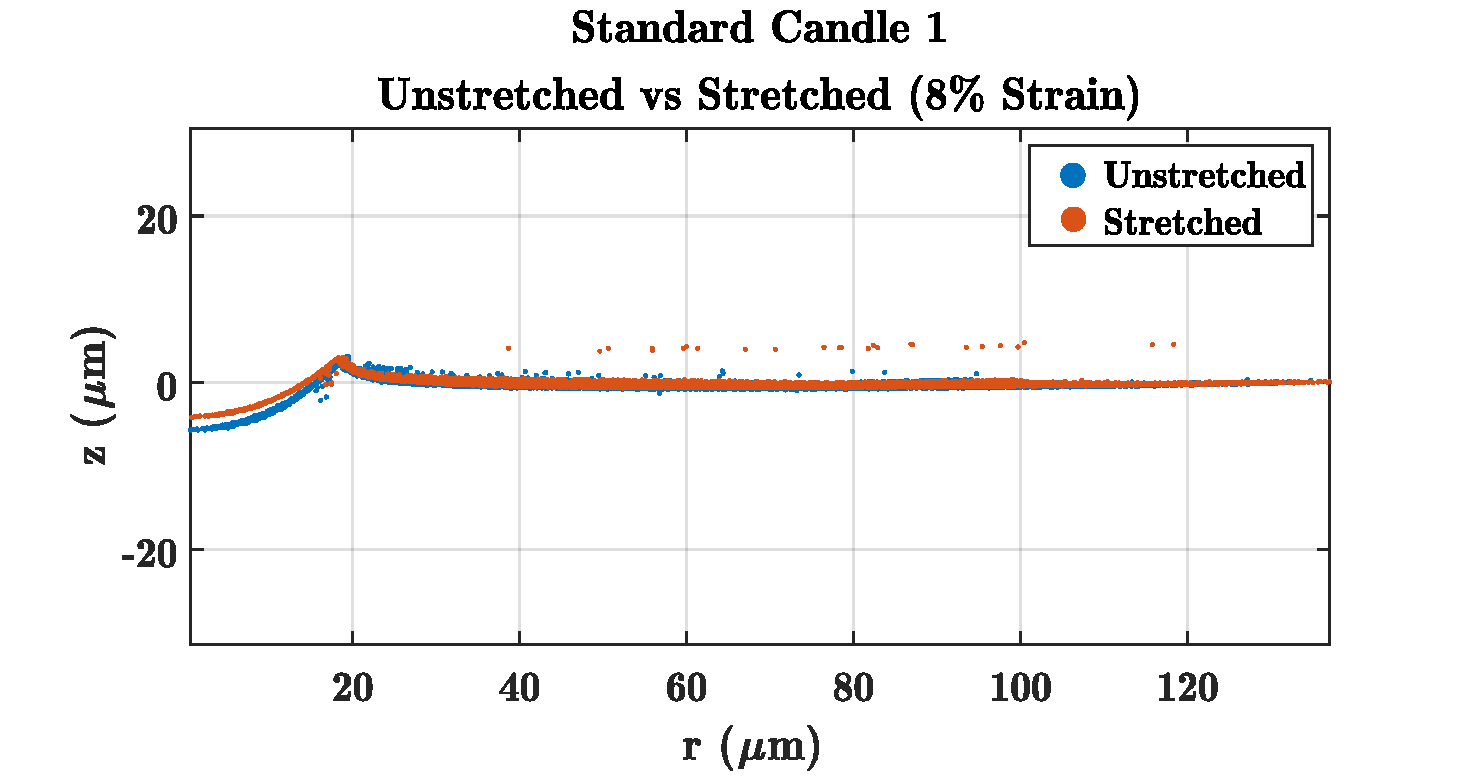
\includegraphics[width=\linewidth]{Chapters/Figures/sc1_unstretched_v_8ml}
	\caption[Side Collapse Comparison]{The side profile of the same silica sphere sitting in a silicone substrate before and after stretch. When a strain is applied, the sphere's indentation into the substrate is shallower. Substrate is Gelest PDMS with stiffness $\text{E}=6.3$ kPa.}	
	\label{fig:sc1unstretchedv8ml}
\end{figure}

\todo[inline, color=yellow]{I will continue to update this section. I hope to have a much more compelling graph to share, one more similar to Figure 1.}

%From Charlie:
%Your executive summary will give a detailed summary of your thesis, hitting the high points and perhaps including a figure or two.  This should have all of the important take-home messages; though details will of course be left for the thesis itself, here you should give enough detail for a reader to have a good idea of the content of the full document.  Importantly, this summary should be able to stand alone, separate from the rest of the document, so although you will be emphasizing the key results of your work, you will probably also want to include a sentence or two of introduction and context for the work you have done.


